%This template was made by Drexl Spivey
%It is a derived from the IEEE Standard 830-1998 for writing
%Software Requirements Specifications

\chapter{Software Requirments Specifications}
\section{Introduction}
%The introduction of the SRS should provide an overview of the entire SRS. It should contain the following
%subsections:
%a) Purpose;
%b) Scope;
%c) Definitions, acronyms, and abbreviations;
%d) References;
%e) Overview.

\subsection{Purpose}
%This subsection should
%a) Delineate the purpose of the SRS;
%b) Specify the intended audience for the SRS.
\paragraph{This document will describe the entire software development process, including use cases, personas, diagrams, and the end goals of the system. The audience for this document will be any persons interested in the software engineering process used for this project, but more specifically, those responsible for overseeing and rating this project.}



\subsection{Scope}
%This subsection should
%a) Identify the software product(s) to be produced by name (e.g., Host DBMS, Report Generator, etc.);
%b) Explain what the software product(s) will, and, if necessary, will not do;
%c) Describe the application of the software being specified, including relevant benefits, objectives, and goals;
%d) Be consistent with similar statements in higher-level specifications (e.g., the system requirements specification), if they exist.
\paragraph{The name for this product will be "Thunderbird: One Time Password." This product will be a Thunderbird add-on, that will encipher plain text into cipher text, which will be delivered by the Thunderbird client to another Thunderbird recipient, that also has the add-on installed. Finally, the second person will be able to decipher the cipher text back to plain text, and read the message.}

\subsection{Definitions, acronyms, abbreviations}
%This subsection should provide the definitions of all terms, acronyms, and abbreviations required to properly interpret the SRS. This information may be provided by reference to one or more appendixes in the SRS or by reference to other documents.
\paragraph{The following definitions, acronyms, and abbreviations may be used with in the software development process:}

\begin{description}[font=\sffamily\bfseries, leftmargin=1cm]
  \item[client] Refers to an email client, more specifically Mozilla's Thunderbird email client.
  \item[E2EE] End-to-end encrypted, in this case, an end-to-end encrypted email.
  \item[JS] JavaScript.
  \item[AES] Advanced Encryption Standard.
  \item[IEEE] Institute of Electrical and Electronics Engineers.
  \item[asymmetric encryption] Encryption that only uses one key for encryption.
  \item[symmetric encryption] Encryption that requires two keys, one on each side of the private message exchange.
  \item[API] application programming interface.
  \item[extensions] An extension adds features and functions to a browser.
  \item[plain text] The text that we wish to encrypt.
  \item[cipher text] The encrypted text.
  \item[ECB] Electronic Codebook, a AES encryption mode.
  \item[CBC] Cipher Block Chaining, a AES encryption mode.
  \item[CFB] Cipher Feedback Mode, a AES encryption mode.
  \item[OFB] Output Feedback Mode, a AES encryption mode.
  \item[CTR] Counter Mode, a AES encryption mode.
  \item[SRS] Software Requirements Specification.
\end{description}

\subsection{References}
%This subsection should
%a) Provide a complete list of all documents referenced elsewhere in the SRS;
%b) Identify each document by title, report number (if applicable), date, and publishing organization;
%c) Specify the sources from which the references can be obtained.
%
%This information may be provided by reference to an appendix or to another document
\paragraph{Author used the IEEE document:}
\begin{enumerate}
\item IEEE Std 803-1998
\end{enumerate}
\paragraph{the IEEE Recommended Practice for Software Requirements Specifications.}\footnote{https://cse.msu.edu/~cse870/IEEEXplore-SRS-template.pdf}

\subsection{Overview}
%This subsection should
%a) Describe what the rest of the SRS contains;
%b) Explain how the SRS is organized.

\section{Overall Description}
%This section of the SRS should describe the general factors that affect the product and its requirements. This
%section does not state specific requirements. Instead, it provides a background for those requirements, which
%are defined in detail in Section 3 of the SRS, and makes them easier to understand.
%This section usually consists of six subsections, as follows:
%a) Product perspective;
%b) Product functions;
%c) User characteristics;
%d) Constraints;
%e) Assumptions and dependencies;
%f) Apportioning of requirements.
\paragraph{The following subsections will describe the general factors that will influence the product requirements, including any background information.}
 
\subsection{Product perspective}
%This subsection of the SRS should put the product into perspective with other related products. If the product is independent and totally self-contained, it should be so stated here. If the SRS defines a product that is a component of a larger system, as frequently occurs, then this subsection should relate the requirements of that larger system to functionality of the software and should identify interfaces between that system and the software.
%
%A block diagram showing the major components of the larger system, interconnections, and external inter-
%faces can be helpful.
%
%This subsection should also describe how the software operates inside various constraints. For example,
%these constraints could include
%a) System interfaces;
%b) User interfaces;
%c) Hardware interfaces;
%d) Software interfaces;
%e) Communications interfaces;
%f) Memory;
%g) Operations;
%h) Site adaptation requirements.
\paragraph{The developed software product, \emph{Thunderbird: One Time Password}, has not current rival. It current alternatives would be Mozilla's own implementation of OpenPGP. The previous option was PgP through the add-on Enigmail. However, at the writing of this document, the add-on is no longer supported.}
\paragraph{The two alternatives do have the advantage that they used symmetric key exchange to encrypt emails, which is more secure, and recommended for encoded email exchange. The \emph{Thunderbird: One Time Password} add-on will have the feature that it is easy to use, at the expense of security.}


\subsubsection{System interfaces}
%This should list each system interface and identify the functionality of the software to accomplish the system requirement and the interface description to match the system.
\paragraph{The required, and assumed interfaces required for the product include the following:}
\begin{enumerate}
\item A modern system, running one of three operating systems:
\begin{enumerate}
\item Windows 10 or later
\item Apple running Big Sur or later
\item Linux variant, running a modern system
\end{enumerate}
\item an Internet connection
\end{enumerate}


\subsubsection{User interfaces}
%This should specify the following:
%a) The logical characteristics of each interface between the software product and its users. This
%includes those configuration characteristics (e.g., required screen formats, page or window layouts,
%content of any reports or menus, or availability of programmable function keys) necessary to accomplish the software requirements.
%b) All the aspects of optimizing the interface with the person who must use the system. This may simply
%comprise a list of do's and dont's on how the system will appear to the user. One example may be a
%requirement for the option of long or short error messages. Like all others, these requirements
%should be verifiable, e.g., a clerk typist grade 4 can do function X in Z min after 1 h of training
%rather than a typist can do function X. (This may also be specified in the Software System
%Attributes under a section titled Ease of Use.)
\paragraph{There are no special user interface requirements.}

\subsubsection{Hardware interfaces}
%This should specify the logical characteristics of each interface between the software product and the hardware components of the system. This includes configuration characteristics (number of ports, instruction sets, etc.). It also covers such matters as what devices are to be supported, how they are to be supported, and protocols. For example, terminal support may specify full-screen support as opposed to line-by-line support.
\paragraph{There are no special hardware interfaces required for this product to function.}

\subsubsection{Software interfaces}
%This should specify the use of other required software products (e.g., a data management system, an operating system, or a mathematical package), and interfaces with other application systems (e.g., the linkage between an accounts receivable system and a general ledger system). For each required software product, the following should be provided:
%
%\begin{enumerate}
%\item Name
%\item Mnemonic
%\item Specification number
%\item Version number
%\item Source
%\end{enumerate}
%
%For each interface, the following should be provided:
%\begin{enumerate}
%\item Discussion of the purpose of the interfacing software as related to this software product.
%\item Definition of the interface in terms of message content and format. It is not necessary to detail any well-documented interface, but a reference to the document defining the interface is required.
%\end{enumerate}

\paragraph{The required software interfaces are:}
\begin{enumerate}
\item Mozilla's free, open source email client, Thunderbird, to be installed on the system.
\item The client should be configured to send and receive emails.\footnote{Thus, an email account on an email server is assumed.}
\item The client should be updated to the latest current software version.
\item The client can be installed on any current (or recent) Windows, Linux, or Apple OS.\footnote{No other OS will be tested.}
\end{enumerate}



\subsubsection{Communications interfaces}
%This should specify the various interfaces to communications such as local network protocols, etc.
\paragraph{No special communication interfaces will be required, than would already be prerequisites for Email communication, i.e. network capable computer.}

\subsubsection{Memory constraints}
%This should specify any applicable characteristics and limits on primary and secondary memory.
\paragraph{Not applicable}


\subsubsection{Operations}
%This should specify the normal and special operations required by the user such as
%a) The various modes of operations in the user organization (e.g., user-initiated operations);
%b) Periods of interactive operations and periods of unattended operations;
%c) Data processing support functions; 
%d) Backup and recovery operations.
%
%NOTE - This is sometimes specified as part of the User Interfaces section.
\paragraph{Not applicable}

\subsubsection{Site adaptation requirements}
%This should
%a) Define the requirements for any data or initialization sequences that are specific to a given site,
%mission, or operational mode (e.g., grid values, safety limits, etc.);
%b) Specify the site or mission-related features that should be modified to adapt the software to a particular installation.
\paragraph{Not applicable}






\subsection{Product functions}
%This subsection of the SRS should provide a summary of the major functions that the software will perform.
%For example, an SRS for an accounting program may use this part to address customer account maintenance,
%customer statement, and invoice preparation without mentioning the vast amount of detail that each of those functions requires.
%Sometimes the function summary that is necessary for this part can be taken directly from the section of the higher-level specification (if one exists) that allocates particular functions to the software product. Note that for the sake of clarity
%a) The functions should be organized in a way that makes the list of functions understandable to the
%customer or to anyone else reading the document for the first time.
%b) Textual or graphical methods can be used to show the different functions and their relationships.
%Such a diagram is not intended to show a design of a product, but simply shows the logical relation-
%ships among variables.



\subsection{User characteristics}
%This subsection of the SRS should describe those general characteristics of the intended users of the product including educational level, experience, and technical expertise. It should not be used to state specific requirements, but rather should provide the reasons why certain specific requirements are later specified in Section 3 of the SRS.

\subsection{Constraints}
%This subsection of the SRS should provide a general description of any other items that will limit the developer's options. These include:
%a) Regulatory policies;
%b) Hardware limitations (e.g., signal timing requirements);
%c) Interfaces to other applications;
%d) Parallel operation;
%e) Audit functions;
%f) Control functions;
%g) Higher-order language requirements;
%h) Signal handshake protocols (e.g., XON-XOFF, ACK-NACK);
%i) Reliability requirements;
%j) Criticality of the application;
%k) Safety and security considerations.
\paragraph{There will be various constraints within this project listed below:}
\begin{itemize}
\item Security: It will not be possible to account for all attack vectors. Thus, only known, common attack vectors will be discussed.
\item Security: How Mallory comes into possession of an encrypted email may not be fully explored. Related to 1. above, but we'll at least give an examination to this possibility -- however she came into possess the Email.
\end{itemize}


\subsection{Assumptions and dependencies}
%This subsection of the SRS should list each of the factors that affect the requirements stated in the SRS.
%These factors are not design constraints on the software but are, rather, any changes to them that can affect the requirements in the SRS. For example, an assumption may be that a specific operating system will be available on the hardware designated for the software product. If, in fact, the operating system is not available, the SRS would then have to change accordingly.

% Not sure what to do with this??
%5.2.6 Apportioning of requirements (2.6 of the SRS)
%This subsection of the SRS should identify requirements that may be delayed until future versions of the
%system.


\section{Specific Requirements}
%This section of the SRS should contain all of the software requirements to a level of detail sufficient to
%enable designers to design a system to satisfy those requirements, and testers to test that the system satisfies those requirements. Throughout this section, every stated requirement should be externally perceivable by users, operators, or other external systems. These requirements should include at a minimum a description of every input (stimulus) into the system, every output (response) from the system, and all functions performed by the system in response to an input or in support of an output. As this is often the largest and most important part of the SRS, the following principles apply:
%a) Specific requirements should be stated in conformance with all the characteristics described in 4.3.
%b) Specific requirements should be cross-referenced to earlier documents that relate.
%c) All requirements should be uniquely identifiable.
%d) Careful attention should be given to organizing the requirements to maximize readability.

%Before examining specific ways of organizing the requirements it is helpful to understand the various items that comprise requirements as described in 5.3.1 through 5.3.7.

\input{UseCaseTemplate}

%% Use Case Diagrams

%TODO These are pretty junk - fix or remove later

\subsection{Use Case Diagrams}

%\begin{wrapfigure}{R}{0.3\textwidth}
%\begin{center}
%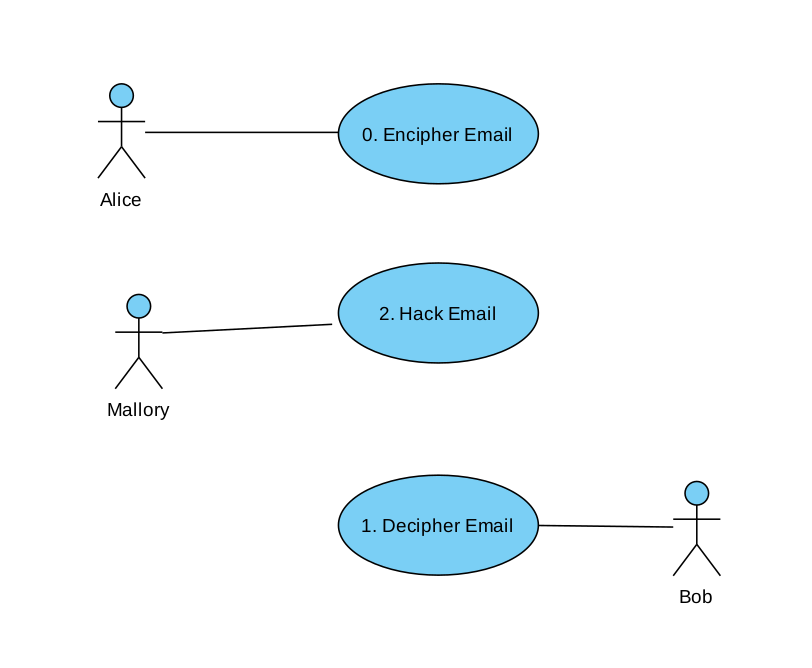
\includegraphics[scale=.50]{useCaseDiagram.png}
%\end{center}
%\end{wrapfigure}

\begin{figure}
    \centering
    \textbf{Use Case Diagrams}\par\medskip
    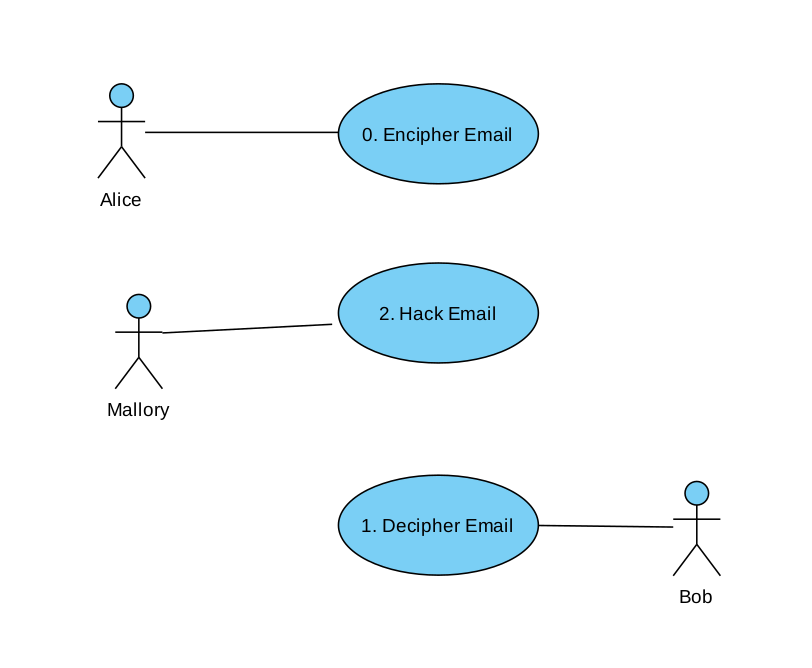
\includegraphics[scale=0.5]{useCaseDiagram.png}
%    \caption{Your caption}
\end{figure}

\section{Appendix}
%The appendixes are not always considered part of the actual SRS and are not always necessary. They may
%include
%a) Sample input/output formats, descriptions of cost analysis studies, or results of user surveys;
%b) Supporting or background information that can help the readers of the SRS;
%c) A description of the problems to be solved by the software;
%d) Special packaging instructions for the code and the media to meet security, export, initial loading, or
%other requirements.
%
%When appendixes are included, the SRS should explicitly state whether or not the appendixes are to be
%considered part of the requirements.


%%These were added in this particular project.
%% This tex file holds the personas png images made with another
% external website/program
\newpage
\subsection{Personas}

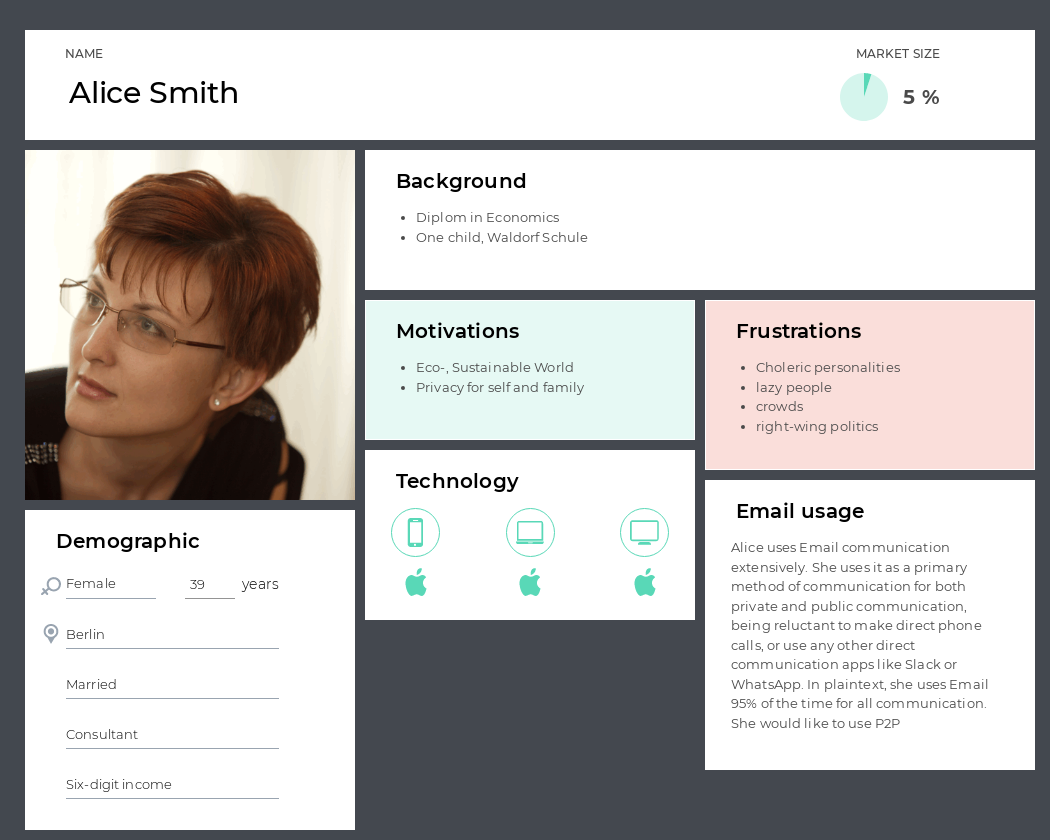
\includegraphics[scale=.38]{Alice Smith.png}
\\
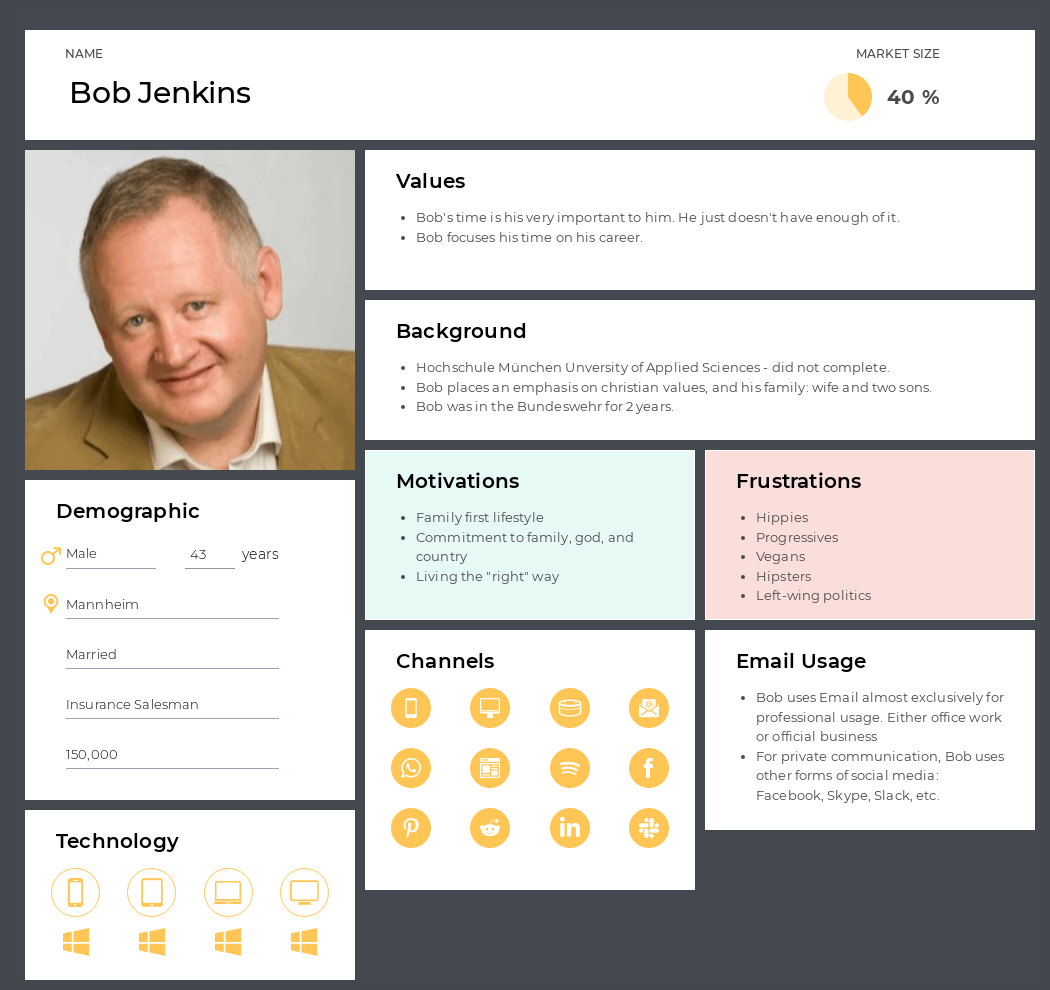
\includegraphics[scale=.38]{Bob Jenkins.png}

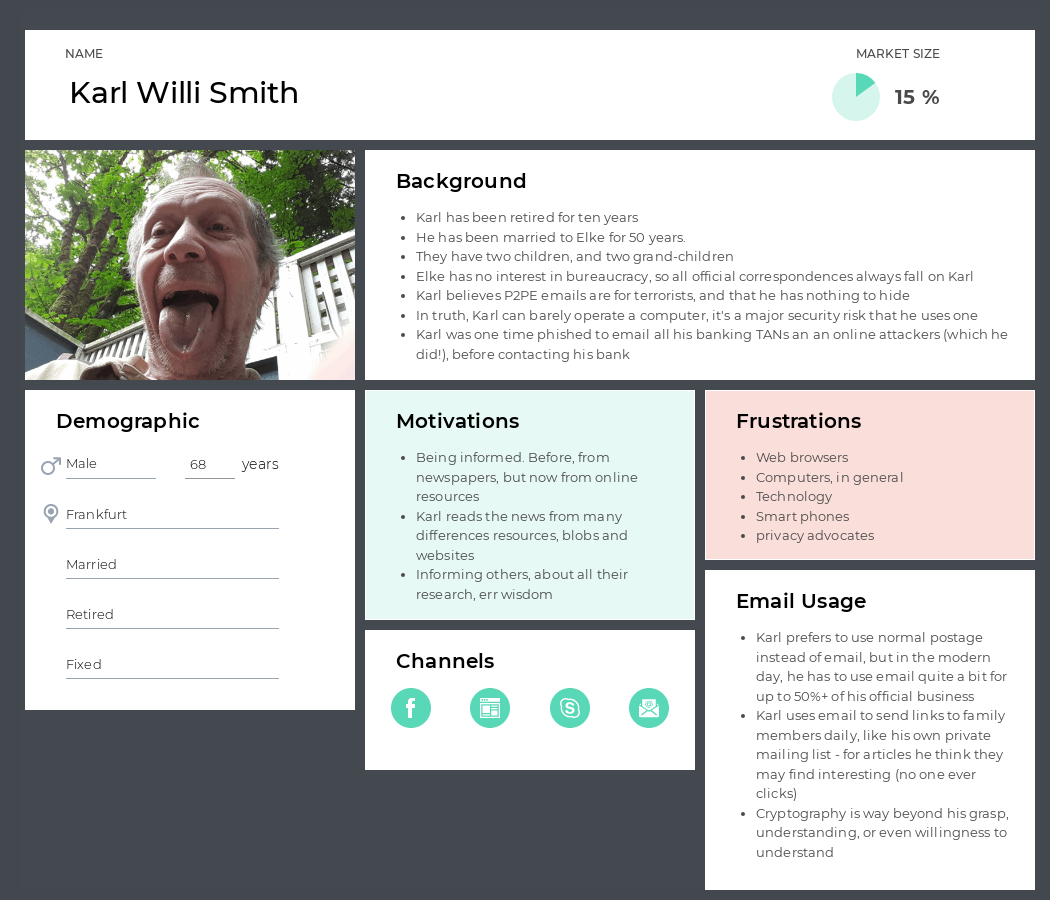
\includegraphics[scale=.38]{Karl Willi Smith.png}

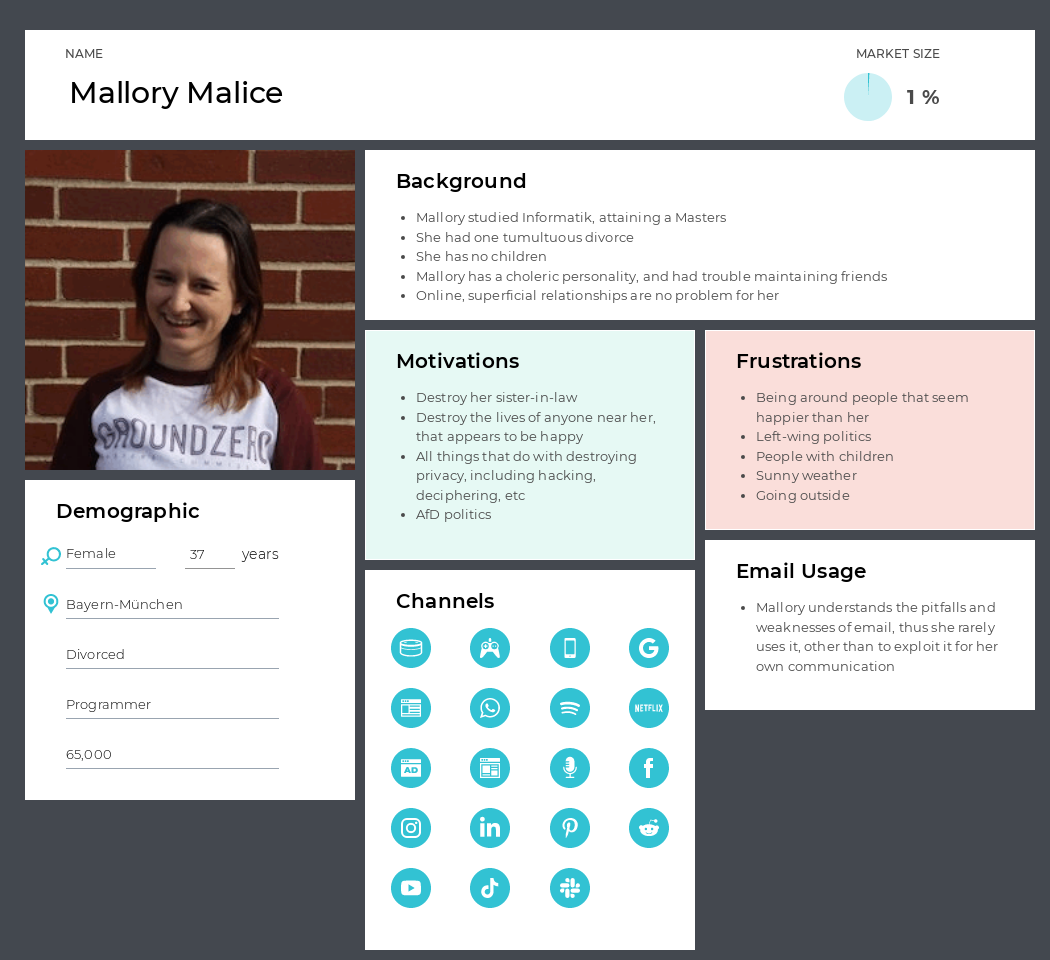
\includegraphics[scale=.38]{Mallory Malice.png}





%\section{Index} I don't know what purpose this is supposed to serve, and it's not clearly stated in the document, so I am leaving it out for now.